% case name
\chapter{Coupling \telemac{3D} with AED2 in a basin (waq3d\_aed2)}
%
% - Purpose & Description:
%     These first two parts give reader short details about the test case,
%     the physical phenomena involved, the geometry and specify how the numerical solution will be validated
%
\section{Purpose}
%
This test shows the coupling between \telemac{3D} and the water quality library AED2.
%
\section{Description}
%
A perfectly still basin is considered (length 1~m, width 1~m, and constant water
depth 5~m) with flat bottom ($z$ = 0~m).
%
\section{Computational options}
%
\subsection{Mesh}
%
The triangular mesh is composed of 49 triangular elements and 36 nodes
(see Figure \ref{fig:waq3d_aed2:mesh}).

\begin{figure}[H]
%\begin{minipage}[t]{0.6\textwidth}
 \centering
 \includegraphicsmaybe{[width=0.6\textwidth]}{../img/res_mesh.png}
%\end{minipage}
\caption{Horizontal mesh}
 \label{fig:waq3d_aed2:mesh}
\end{figure}

To build the 3D mesh of prisms, 11 planes are regularly spaced over the vertical.
The vertical mesh between nodes of coordinates (0 ; 0.5) to (1 ; 0.5) can be seen
on Figure \ref{fig:waq3d_aed2:mesh_section}.

\begin{figure}[H]
%\begin{minipage}[t]{0.15\textwidth}
 \centering
 \includegraphicsmaybe{[width=0.35\textwidth]}{../img/res_mesh_section.png}
%\end{minipage}
\caption{Vertical mesh}
 \label{fig:waq3d_aed2:mesh_section}
\end{figure}

%\begin{figure} [H]
%\centering
%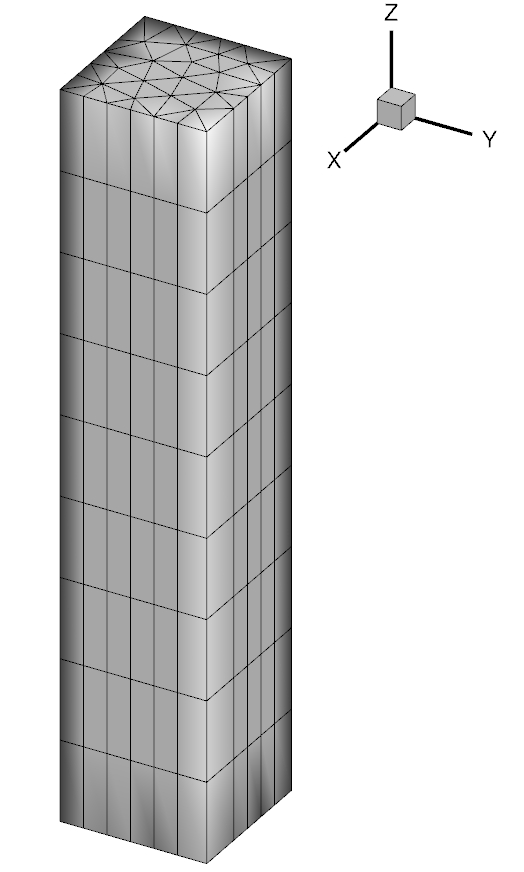
\includegraphics[scale=0.4]{mesh_waq3d-aed2.jpg}
% \caption{waq3d\_aed2 test: horizontal and vertical meshes}
% \label{fig:waq3d_aed2:3Dmesh}
%\end{figure}
%
%\subsection{Physical parameters}
%
\subsection{Water quality parameters}
Coupling with \waqtel and water quality processes = 13 (AED2),
aed2.nml file contains the AED2 parametrization.
The following modules are activated:
\begin{itemize}
\item sedflux,
\item oxygen,
\item carbon,
\item silica,
\item nitrogen,
\item phosphorus,
\item organic matter,
\item phytoplankton,
\item tracer.
\end{itemize}

As there are 25 tracers taken into account, the value of
\telkey{MAXIMUM NUMBER OF TRACERS} has to be inscreased compared to its default
value (20).
%
\subsection{Initial and Boundary Conditions}
%
The initial water depth is 5~m with a fluid at rest.\\
The initial concentrations are homogeneous.\\

There are only closed lateral boundaries with free slip condition and
Nikuradse law is used to model friction at the bottom with a coefficient
0.001~m.
%
\subsection{General parameters}
%
The time step is 1~s for a simulated period of 1,000~s.
%
\subsection{Numerical parameters}
%
The non-hydrostatic version of \telemac{3D} is used (default option).
The LIPS scheme is chosen to solve the advection for the tracers
(default option).
But as the fluid is at rest, no specific effects can be seen.
%
\subsection{Comments}
Among the tracers, only the temperature, oxygen (O$_2$), ammonium (NH$_4$),
nitrate (NO$_3$), phosphate (PO$_4$), Dissolved Organic Phosphorus (DOP),
Dissolved Organic Nitrogen (DON) and Particulate Organic Phosphorus (POP)
concentrations are written in the result files for this example.

% - Results:
%     We comment in this part the numerical results against the reference ones,
%     giving understanding keys and making assumptions when necessary.
%
\section{Results}

As an example, Figure \ref{fig:waq3d_aed2:res} shows the oxygen, ammonium,
nitrate, phosphate, DOP, DON concentrations at the end of the calculation
in a vertical section.
They vary in the water column.
Temperature and POP remain homogeneous in the domain.

%Depending on exchange with sediments, concentrations evolve in a good manner.

%\begin{figure} [H]
%\centering
%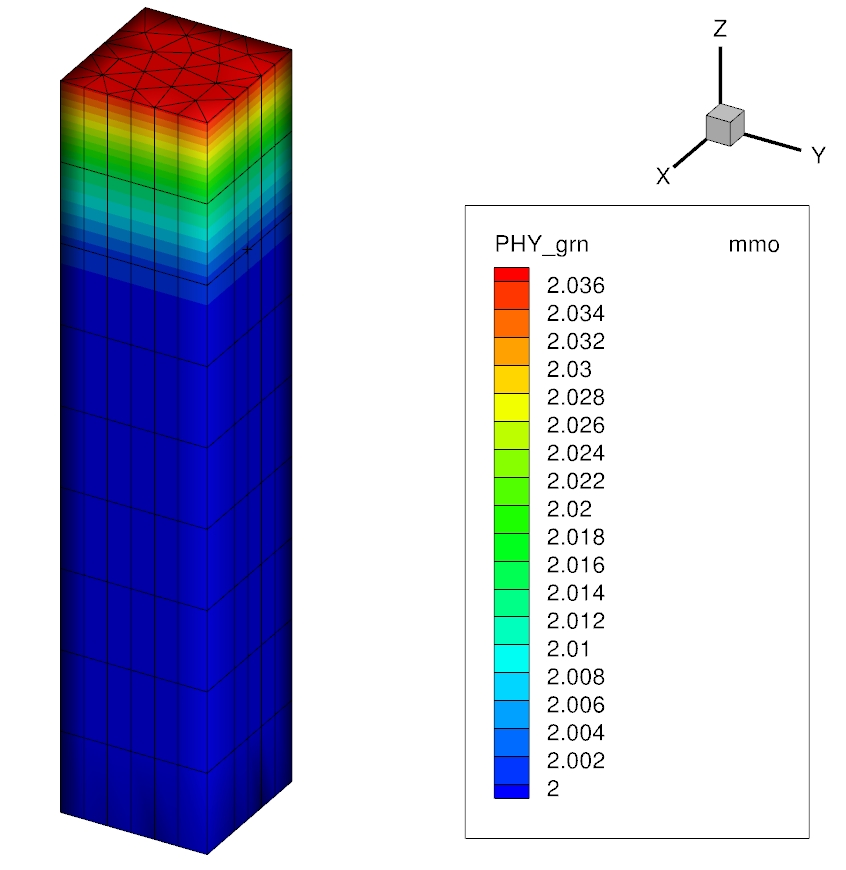
\includegraphics[scale=0.4]{phyto.jpg}
% \caption{waq3d aed2 test: phytoplankton concentration after 1,000s.}
% \label{fig:waq3d_aed2:res}
%\end{figure}

\begin{figure}[H]
\centering
\begin{minipage}[t]{0.3\textwidth}
 \centering
\includegraphicsmaybe{[width=\textwidth]}{../img/res_oxy.png}
\end{minipage}
%
\begin{minipage}[t]{0.3\textwidth}
 \centering
\includegraphicsmaybe{[width=\textwidth]}{../img/res_ammonium.png}
\end{minipage}
%
\begin{minipage}[t]{0.3\textwidth}
 \centering
\includegraphicsmaybe{[width=\textwidth]}{../img/res_nitrate.png}
\end{minipage}
%
\begin{minipage}[t]{0.3\textwidth}
 \centering
\includegraphicsmaybe{[width=\textwidth]}{../img/res_phosphate.png}
\end{minipage}
%
\begin{minipage}[t]{0.3\textwidth}
 \centering
\includegraphicsmaybe{[width=\textwidth]}{../img/res_dop.png}
\end{minipage}
%
\begin{minipage}[t]{0.3\textwidth}
 \centering
\includegraphicsmaybe{[width=\textwidth]}{../img/res_don.png}
\end{minipage}
%
 \caption{Vertical distribution of oxygen, ammonium, nitrate, phosphate, DOP, DON (from left to right then top to bottom at the end of computation)}
 \label{fig:waq3d_aed2:res}
\end{figure}
%
\section{Conclusion}
%
\telemac{3D} can be coupled with AED2 to model water quality processes.
%
% Here is an example of how to include the graph generated by validate_telemac.py
% They should be in test_case/img
%\begin{figure} [!h]
%\centering
%\includegraphics[scale=0.3]{../img/mygraph.png}
% \caption{mycaption}\label{mylabel}
%\end{figure}
